%% History:
% Pavel Tvrdik (26.12.2004)
%  + initial version for PhD Report
%
% Daniel Sykora (27.01.2005)
%
% Michal Valenta (3.12.2008)
% rada zmen ve formatovani (diky M. Duškovi, J. Holubovi a J. Žďárkovi)
% sjednoceni zdrojoveho kodu pro anglickou, ceskou, bakalarskou a diplomovou praci

% One-page layout: (proof-)reading on display
%%%% \documentclass[11pt,oneside,a4paper]{book}
% Two-page layout: final printing
\documentclass[11pt,twoside,a4paper]{book}   
%=-=-=-=-=-=-=-=-=-=-=-=--=%
% The user of this template may find useful to have an alternative to these 
% officially suggested packages:
\usepackage[czech, english]{babel}
\usepackage[T1]{fontenc} % pouzije EC fonty 
% pripadne pisete-li cesky, pak lze zkusit take:
% \usepackage[OT1]{fontenc} 
\usepackage[utf8]{inputenc}
%=-=-=-=-=-=-=-=-=-=-=-=--=%
% In case of problems with PDF fonts, one may try to uncomment this line:
%\usepackage{lmodern}
%=-=-=-=-=-=-=-=-=-=-=-=--=%
%=-=-=-=-=-=-=-=-=-=-=-=--=%
% Depending on your particular TeX distribution and version of conversion tools 
% (dvips/dvipdf/ps2pdf), some (advanced | desperate) users may prefer to use 
% different settings.
% Please uncomment the following style and use your CSLaTeX (cslatex/pdfcslatex) 
% to process your work. Note however, this file is in UTF-8 and a conversion to 
% your native encoding may be required. Some settings below depend on babel 
% macros and should also be modified. See \selectlanguage \iflanguage.
% \usepackage{czech}  %%%%%\usepackage[T1]{czech} %%%%[IL2] [T1] [OT1]
%=-=-=-=-=-=-=-=-=-=-=-=--=%

%%%%%%%%%%%%%%%%%%%%%%%%%%%%%%%%%%%%%%%
% Styles required in your work follow %
%%%%%%%%%%%%%%%%%%%%%%%%%%%%%%%%%%%%%%%
\usepackage{graphicx}
%\usepackage{indentfirst} %1. odstavec jako v cestine.

\usepackage{k336_thesis_macros} % specialni makra pro formatovani DP a BP
 % muzete si vytvorit i sva vlastni v souboru k336_thesis_macros.sty
 % najdete  radu jednoduchych definic, ktere zde ani nejsou pouzity
 % napriklad: 
 % \newcommand{\bfig}{\begin{figure}\begin{center}}
 % \newcommand{\efig}{\end{center}\end{figure}}
 % umoznuje pouzit prikaz \bfig namisto \begin{figure}\begin{center} atd.
\usepackage{amssymb,amsmath}

%%%%%%%%%%%%%%%%%%%%%%%%%%%%%%%%%%%%%
% Zvolte jednu z moznosti 
% Choose one of the following options
%%%%%%%%%%%%%%%%%%%%%%%%%%%%%%%%%%%%%
% \newcommand\TypeOfWork{Diplomová práce} \typeout{Diplomova prace}
% \newcommand\TypeOfWork{Master's Thesis}   \typeout{Master's Thesis} 
\newcommand\TypeOfWork{Bakalářská práce}  \typeout{Bakalarska prace}
% \newcommand\TypeOfWork{Bachelor's Project}  \typeout{Bachelor's Project}


%%%%%%%%%%%%%%%%%%%%%%%%%%%%%%%%%%%%%
% Zvolte jednu z moznosti 
% Choose one of the following options
%%%%%%%%%%%%%%%%%%%%%%%%%%%%%%%%%%%%%
% nabidky jsou z: http://www.fel.cvut.cz/cz/education/bk/prehled.html

\newcommand\StudProgram{Elektrotechnika a informatika, dobíhající, Bakalářský}
% \newcommand\StudProgram{Elektrotechnika a informatika, dobíhající, Magisterský}
% \newcommand\StudProgram{Elektrotechnika a informatika, strukturovaný, Bakalářský}
% \newcommand\StudProgram{Elektrotechnika a informatika, strukturovaný, Navazující magisterský}
% \newcommand\StudProgram{Softwarové technologie a management, Bakalářský}
% English study:
% \newcommand\StudProgram{Electrical Engineering and Information Technology}  % bachelor programe
% \newcommand\StudProgram{Electrical Engineering and Information Technology}  %master program


%%%%%%%%%%%%%%%%%%%%%%%%%%%%%%%%%%%%%
% Zvolte jednu z moznosti 
% Choose one of the following options
%%%%%%%%%%%%%%%%%%%%%%%%%%%%%%%%%%%%%
% nabidky jsou z: http://www.fel.cvut.cz/cz/education/bk/prehled.html

\newcommand\StudBranch{Výpočetní technika}   % pro program EaI bak. (dobihajici i strukt.)
% \newcommand\StudBranch{Výpočetní technika}   % pro prgoram EaI mag. (dobihajici i strukt.)
% \newcommand\StudBranch{Softwarové inženýrství}            %pro STM
% \newcommand\StudBranch{Web a multimedia}                  % pro STM
% \newcommand\StudBranch{Computer Engineering}              % bachelor programe
% \newcommand\StudBranch{Computer Science and Engineering}  % master programe


%%%%%%%%%%%%%%%%%%%%%%%%%%%%%%%%%%%%%%%%%%%%
% Vyplnte nazev prace, autora a vedouciho
% Set up Work Title, Author and Supervisor
%%%%%%%%%%%%%%%%%%%%%%%%%%%%%%%%%%%%%%%%%%%%

\newcommand\WorkTitle{Galerie fotografií s exportem na webové stránky }
\newcommand\FirstandFamilyName{Pavel Macenauer}
\newcommand\Supervisor{Doc. Ing. Jan Janoušek Ph.D.}


% Pouzijete-li pdflatex, tak je prijemne, kdyz bude mit vase prace
% funkcni odkazy i v pdf formatu
\usepackage[
pdftitle={\WorkTitle},
pdfauthor={\FirstandFamilyName},
bookmarks=true,
colorlinks=true,
breaklinks=true,
urlcolor=red,
citecolor=blue,
linkcolor=blue,
unicode=true,
]
{hyperref}



% Extension posted by Petr Dlouhy in order for better sources reference (\cite{} command) especially in Czech.
% April 2010
% See comment over \thebibliography command for details.

\usepackage[square, numbers]{natbib}             % sazba pouzite literatury
%\usepackage{url}
%\DeclareUrlCommand\url{\def\UrlLeft{<}\def\UrlRight{>}\urlstyle{tt}}  %rm/sf/tt
%\renewcommand{\emph}[1]{\textsl{#1}}    % melo by byt kurziva nebo sklonene,
\let\oldUrl\url
\renewcommand\url[1]{<\texttt{\oldUrl{#1}}>}




\begin{document}

%%%%%%%%%%%%%%%%%%%%%%%%%%%%%%%%%%%%%
% Zvolte jednu z moznosti 
% Choose one of the following options
%%%%%%%%%%%%%%%%%%%%%%%%%%%%%%%%%%%%%
\selectlanguage{czech}
%\selectlanguage{english} 

% prikaz \typeout vypise vyse uvedena nastaveni v prikazovem okne
% pro pohodlne ladeni prace

\iflanguage{czech}{
	 \typeout{************************************************}
	 \typeout{Zvoleny jazyk: cestina}
	 \typeout{Typ prace: \TypeOfWork}
	 \typeout{Studijni program: \StudProgram}
	 \typeout{Obor: \StudBranch}
	 \typeout{Jmeno: \FirstandFamilyName}
	 \typeout{Nazev prace: \WorkTitle}
	 \typeout{Vedouci prace: \Supervisor}
	 \typeout{***************************************************}
	 \newcommand\Department{Katedra počítačů}
	 \newcommand\Faculty{Fakulta elektrotechnická}
	 \newcommand\University{České vysoké učení technické v Praze}
	 \newcommand\labelSupervisor{Vedoucí práce}
	 \newcommand\labelStudProgram{Studijní program}
	 \newcommand\labelStudBranch{Obor}
}{
	 \typeout{************************************************}
	 \typeout{Language: english}
	 \typeout{Type of Work: \TypeOfWork}
	 \typeout{Study Program: \StudProgram}
	 \typeout{Study Branch: \StudBranch}
	 \typeout{Author: \FirstandFamilyName}
	 \typeout{Title: \WorkTitle}
	 \typeout{Supervisor: \Supervisor}
	 \typeout{***************************************************}
	 \newcommand\Department{Department of Computer Science and Engineering}
	 \newcommand\Faculty{Faculty of Electrical Engineering}
	 \newcommand\University{Czech Technical University in Prague}
	 \newcommand\labelSupervisor{Supervisor}
	 \newcommand\labelStudProgram{Study Programme} 
	 \newcommand\labelStudBranch{Field of Study}
}




%%%%%%%%%%%%%%%%%%%%%%%%%%    Titulni stranka / Title page 

\coverpagestarts

%%%%%%%%%%%%%%%%%%%%%%%%%%%    Podekovani / Acknowledgements 

\acknowledgements
\noindent
Chtěl bych poděkovat vedoucímu práce doc. Ing. Janu Janouškovi Ph.D. za podporu a možnost pracovat na bakalářské práci s tématikou zpracování obrazu, která mne velmi zajímá.


%%%%%%%%%%%%%%%%%%%%%%%%%%%   Prohlaseni / Declaration 

\declaration{V~Praze dne 4.\,1.\,2012}


%%%%%%%%%%%%%%%%%%%%%%%%%%%%    Abstract 
 
\abstractpage
\noindent 
The subject of this thesis is GalleryManager, simple image editor and photo-organizer. This cross-platform graphical application organizes pictures into folders called galleries including their full description. Graphic editor allows to carry out simple image editing: rotation-resizing, changes of brightness, contrast and saturation and conversion of coloured images into black and white. Individual galleries and photos can be documented not only by adding names and descriptions, but also with embedded image metadata. Output from the program is a web presentation.

\indent
Focus was given on speed of image processing and possibility to expand the application with additional functionalities. Program supports images in JPEG format and 8-bit colour depth.
% Prace v cestine musi krome abstraktu v anglictine obsahovat i
% abstrakt v cestine.
\vglue50mm

\noindent{\Huge \textbf{Abstrakt}}
\vskip 2.75\baselineskip

\noindent 
Předmětem práce je vytvoření programu GalleryManager pro správu, úpravu a export fotografií. Jedná se o multiplatformní grafickou aplikaci, která slouží k organizaci fotografií do složek označovaných jako galerie a jejich správě. Obsahuje jednoduchý grafický editor umožňující základní obrazové úpravy. Jmenovitě rotaci, zvětšování/zmenšování, barevné úpravy jasu, kontrastu, sytosti a převod barevného obrazu na černobílý. Jednotlivé galerie a fotografie lze dokumentovat a to nejen za pomoci jmenovek a popisků, ale načítají se i obrazová metadata. Výstupem z programu je webová prezentace se zpracovanými fotogaleriemi.

\indent
Důraz při vývoji aplikace byl kladen na rychlost zpracování obrazu a možnost rozšiřovat program o další funkce. Zpracování fotografií probíhá z formátu JPEG v 8-bitové barevné hloubce.



%%%%%%%%%%%%%%%%%%%%%%%%%%%%%%%%  Obsah / Table of Contents 

\tableofcontents

%%%%%%%%%%%%%%%%%%%%%%%%%%%%%%%  Seznam obrazku / List of Figures 

\listoffigures

%%%%%%%%%%%%%%%%%%%%%%%%%%%%%%%  Seznam tabulek / List of Tables

\listoftables

%**************************************************************

\mainbodystarts
% horizontalní mezera mezi dvema odstavci
%\parskip=5pt
%11.12.2008 parskip + tolerance
\normalfont
\parskip=0.2\baselineskip plus 0.2\baselineskip minus 0.1\baselineskip

% Odsazeni prvniho radku odstavce resi class book (neaplikuje se na prvni 
% odstavce kapitol, sekci, podsekci atd.) Viz usepackage{indentfirst}.
% Chcete-li selektivne zamezit odsazeni 1. radku nektereho odstavce,
% pouzijte prikaz \noindent.

%**************************************************************

% Pro snadnejsi praci s vetsimi texty je rozumne tyto rozdelit
% do samostatnych souboru nejlepe dle kapitol a tyto potom vkladat
% pomoci prikazu \include{jmeno_souboru.tex} nebo \include{jmeno_souboru}.
% Napr.:
% \include{1_uvod}
% \include{2_teorie}
% atd...

%*****************************************************************************

\chapter{Úvod}

\noindent
V současné době je na trhu velké množství grafických editorů, programů pro správu fotografií a těch, které kombinují obojí. Z komerčních produktů jsou nejznámější rozsáhlé programové balíky Photoshop a Lightroom od Adobe Systems Inc. V České republice se velmi dobře prosadil i mnohem levnější Zoner Photo Studio. Bezplatně je možné využívat služeb Google Picassa nebo IrfanView. Komerční produkty mají za sebou již mnoho let vývoje a týmy vývojářů.

\indent
Aplikaci jsem pojmenoval GalleryManager. Jedná se o jednoduchý grafickým editor a správce fotografií s možností tvorby popisů. Aplikaci do budoucna plánuji integrovat do správy vlastních webových stránek, zaměřených na cestovatelskou fotografii PhotographicAtlas.com a FotoAtlas.cz. Není zde cílem implementovat pokročilé algoritmy pro úpravu fotografií, které již nabízejí existující softwary, zaměřené na práci s velkými soubory a tisk. Naopak je kladen důraz na rychlost a efektivitu pro potřeby webové prezentace.

\indent
Dokumentární nebo reportážní fotografové, pro které je GalleryManager určen, nespravují své fotografie jednotlivě, ale jako celé série. Cílem je umožnit rychlou práci s více fotografiemi současně a zpřístupnit i neobrazové informace vkládané fotoaparáty do fotografie (například údaje o nastavení fotoaparátu, místě a času pořízení snímku a další).

\indent
Aktuálně je aplikace navržena tak, aby výstupem byla nezávislá webová stránka, kterou lze použít pro vlastní prezentaci na internetu.

\indent
Tato práce je implementační, nikoliv rešeršní, proto dokumentace bude popsána především z programátorského hlediska, popisující postup při tvorbě aplikace a možnosti použitých knihoven. Vzhledem k tomu, že bych se i do budoucna chtěl věnovat úpravám obrazu a nadále rozšiřovat aplikaci o další možnosti, budou popsány jednotlivé algoritmy pro úpravu fotografií, jejich výhody, nevýhody a srovnání s jinými obecně známými.

%*****************************************************************************

\chapter{Popis problému, specifikace cíle}
\section{Cíle práce}

\noindent
Hlavním cílem této práce je vytvořit grafický editor, který umožní organizovat, popisovat a nakonec exportovat fotografie do podoby webové prezentace. Nejedná se o práci, která bude prezentována jako hotový program, ale spíše jako framework pro správu a úpravy fotografií, který půjde dále rozšiřovat.

\indent
Zpracování obrazu a informací spojených s fotografií je natolik rozsáhlé téma, že přesahuje rozsah bakalářské práce, časové možnosti i znalosti jediného člověka. Cílem aplikace GalleryManager je vytvořit:

\begin{itemize}
\item grafické uživatelské rozhraní
\item stromovou strukturu podsložek (galerií) a jednotlivých fotografií
\item možnost každou galerii a fotografii popisovat, do budoucna by měla být struktura přizpůsobena, aby šla rozšiřovat
\item automatické vkládání informací z EXIF údajů fotografie
\item základní grafické úpravy - jas, kontrast, sytost, transformace obrazu, ...
\item export projektu do standardních formátů - XML, HTML/CSS a možnost ho ukládat a opět načítat
\item multiplatformní podporu aplikace
\end{itemize}

\section{Podoba práce vzhledem k vytyčeným cílům}
\noindent
Jedná se o grafickou aplikaci psanou v jazyce C++. Průběh práce s programem, při zpracování a organizaci vlastních fotografií vypadá takto:
\begin{enumerate}

\item po spuštění programu GalleryManager se spustí prázdný projekt bez jakýchkoliv podsložek
\item uživatel má možnost nahrát projekt, který vytvořil v minulosti, včetně všech podsložek a fotografií
\item v rámci projektu lze vytvářet nové podsložky (galerie) nebo upravovat již existující
\item do existujících nebo nově vytvořených podsložek naimportuje uživatel nové fotografie
	\begin{itemize}
	\item během importu fotografií se načtou a zobrazí EXIF informace
	\item je možné přidávat další popisky
	\item při rozkliknutí složky se zobrazí její obsah - podsložky jako obálky a fotografie jako malé náhledy
	\item při rozkliknutí fotografie se zobrazí fotografie v plném rozlišení v prostředí pro úpravu
	\end{itemize}
\item projekt lze ukládat ve formátu XML
\item projekt lze exportovat ve formátu HTML do podoby webové prezentace, přičemž vzhled se určí pomocí vložené CSS šablony
\item CSS lze libovolně vytvářet na základě popsané HTML struktury, a tak vkládat vlastní design
\end{enumerate}

\section{Existující implementace}
\noindent
Rešerši existujících produktů jsem prováděl v průběhu listopadu a prosince 2011. Lze předpokládat, že se objeví další aplikace a existující produkty budou i nadále rozšiřovány do podoby dalších verzí.

\indent
Programy pro práci s fotografiemi lze rozdělit na aplikace pro správu fotografií a grafické editory. Společností, která vládne v komerční oblasti, je Adobe Systems Inc. Jako multifunkční grafický editor nabízí tato firma Photoshop, jeho odlehčenou verzi Photoshop Elements a balík programů Lightroom, určený téměř výhradně pro fotografy. V České Republice do cenově nižší kategorie zapadá Zoner Photo Studio. Na rozdíl od komerčních aplikací, které se zabývají především pokročilými úpravami obrazu, se nekomerční soustřeďují spíše na organizaci a prohlížení fotografií. K nim lze zařadit Google Picassa, IrfanView a software, přiložený ke správě uživatelského účtu na Rajce.cz. Žádný z těchto programů neposkytuje své zdrojové kódy, proto jediným zdrojem informací jsou uživatelské zkušenosti se samotnými aplikacemi. Zároveň neexistuje ani žádné API, které by umožnilo používat jejich funkce pro vlastní účely.

\subsection{Komerční software}
\noindent
Dnes nejrozsáhlejší softwarový balík Photoshop od společnosti Adobe Systems Inc., prošel za posledních deset let dlouhým vývojem. Umožňuje provádět složité grafické úpravy pomocí práce s vrstvami obrazu, maskami a to nejen výběrovými, ale i kanálovými\footnote{Obraz ve Photoshopu si lze představit jako sendvič složený z jednotlivých obrazových vrstev, které se navzájem prolínají s různou intenzitou, kterou si volí uživatel. Masky, na druhou stranu, jsou uložené výběry, se kterými lze pracovat. Lze takto maskovat nejen plochy, ale i celé barevné kanály}. Na začátku vývoje zpracovával soubory pouze v 8-bitové barevné hloubce. Dnes, hlavně na základě požadavků z oblasti videa, umožňuje práci se soubory ve 32-bitové barevné hloubce (především pro technologii HDR\footnote{High Dynamic Range je technologie umožňující skládat snímky s rozdílnými hodnotami expozice. Jejím praktickým uplatněním je například noční fotografie, kdy chceme zachytit jak kresbu ve světlech, tak i ve tmě.}). Mimo jiné existuje i jeho odlehčená varianta Photoshop Elements, která neobsahuje tolik specializovaných funkcí pro úpravu obrazu.

\indent
Adobe Lightroom je zaměřen na hromadné úpravy fotografických souborů, a to především ve formátech RAW\footnote{Bezkompresní obrazový formát, kterého využívají moderní digitální zrcadlovky k ukládání fotografií v maximálním kvalitě. Je specifický pro každého výrobce.}. Jeho jedinečnost spočívá ve vytváření celých sad grafických úprav, tedy maker, nad více fotografiemi současně. Výhodou je, že se uloží pouze jednotlivá makra úprav a nemění se tak originální soubor. Ten se změní až v okamžiku exportu dat mimo prostředí Lightroom. Umožňuje pouze základní grafické úpravy, v případě složitějších je nucen uživatel přejít do Photoshopu. Nevýhodou je, že jej nelze integrovat do vlastních projektů a napojit ho na vlastní webový server, k čemuž je GalleryManager do budoucna zamýšlen.

\indent
Jako most mezi aplikacemi Adobe slouží Bridge. Dovoluje zobrazovat nejrůznější grafické formáty, včetně jejich organizace. Tento software umožňuje velmi rychle generovat náhledy snímků, někdy na úkor velkého využití místa na disku. Spolupracuje nejen s aplikacemi pro práci s obrazem, tedy s Photoshopem a Lightroomem, ale i s dalšími balíky určenými pro zpracování videa (Premiere, AfterEffects) nebo vektorové grafiky (InDesign, Illustrator).

\indent
Především v České republice je oblíbený Zoner Photo Studio, který se soustředí na to samé jako Adobe Photoshop, tedy grafickou úpravu jednotlivých fotografií. Zdaleka však neobsahuje tolik funkcí. Pro uživatele je atraktivní svou cenou, jednoduchostí a zázemím v České republice.

\subsection{Nekomerční software}
\noindent
Software nabízený zdarma slouží obvykle jako podpora nebo nadstavba služeb poskytovaných webovými servery. Česká webová stránka rajce.cz umožňuje uživatelům sdílet své fotografie v podobě galerií. Poskytuje software, pomocí kterého si uživatel vytvoří galerii, pojmenuje ji, popíše a na svém počítači vybere fotografie, které do ní chce vložit. Zmenšení na náhledy, pro potřebu webové prezentace na www.rajce.cz, provede program automaticky při následném nahrávání. Z grafických úprav lze fotografie otočit o 90 stupňů a pojmenovat. Zatím není možné je jakkoliv upravovat nebo číst jejich EXIF údaje v širším měřítku.

\indent
IrfanView je naopak spíše jednoduchým prohlížečem fotografií. Umožňuje, oproti komerčnímu softwaru, pouze základní grafické úpravy. Jeho hlavní předností a záměrem je zobrazovat fotografie, proto podporuje většinu dnes používaných grafických formátů a umožňuje spustit automatické prohlížení v podobě prezentace.

\indent
Svou koncepcí je GalleryManager asi nejpodobnější produktu Google Picasa, který je se spuštěním sociální sítě Google+ využíván pro synchronizaci fotografií s vlastním uživatelským účtem, ale lze jej používat i samostatně pro grafické úpravy. Galerie se zde vytvářejí přímo v podobě systémových složek, které si Picasa neustále za svého běhu indexuje. Uživatel tak má přehled o všech svých fotografiích na pevném disku. Zajímavé je, že každou chvíli si určitou část využívané paměti uvolní a nezabírá tak velké množství paměti, jaké by člověk očekával od programu, který si neustále vytváří náhledy.

\indent
Sociální sítě dnes slouží především k masovému sdílení vlastních informací. Stejným způsobem pohlíží i Picasa na fotografie. Je přizpůsobena běžnému uživateli, kterému stačí jednoduché úpravy fotografií. Soubory lze synchronizovat s Google+ a prohlížet téměř každý dnes používaný formát. Neumožňuje však načítat všechny informace EXIF. A to především takové, které jsou pro fotografy důležité a dokumentovat tak dostatečně své galerie.

%*****************************************************************************
\bibliographystyle{csplainnat}
%bibliographystyle{plain}
%\bibliographystyle{psc}

\chapter{Analýza a návrh řešení}
\section{Volba programovacích jazyků a knihoven}
\noindent
GalleryManager je prohlížeč fotografií s jednoduchým grafickým editorem. Je navržen tak, aby mohl upravovat a obsluhovat velké množství fotografií paralelně. Potřebujeme tak co nejrychlejší jazyk s velkým množstvím dostupných knihoven, především pro tvorbu GUI, úpravu obrazu a čtení EXIF dat. Zároveň musí být objektově orientovaný a mapovat tak koncept reálného světa. Pro uživatele je důležité vytvářet stromovou strukturu galerií a fotografií o neomezené hloubce, kde každá galerie může v sobě obsahovat opět další galerie a fotografie. 

\indent 
Zvolen byl programovací jazyk C++, který všechny tyto požadavky splňuje. Jeho nevýhodou je, že oproti výše-úrovňovým jazykům jako Java, má zde programátor na starosti i správu paměti a musí velké množství funkcí, které by jinak byly implementovány v základních knihovnách, psát sám.

\indent
Jednotlivé použité knihovny je třeba analyzovat po částech aplikace, kde každá by měla být na druhé co nejméně závislá. Nechceme, aby docházelo k tomu, že při změně části kódu bude třeba přepisovat zbytek aplikace.

\subsection{Grafické uživatelské rozhraní}
\indent
K tvorbě grafického uživatelského rozhraní je použit široce rozšířený framework Qt od Nokie. K jeho výběru vedlo hned několik výhod. Je volně ke stažení pod licencí LGPL v2.1, umožňující volné používání pro nekomerční účely. Z programátorského hlediska má přehlednou dokumentaci, je multiplatformní, tudíž GUI a signály nejsou vázány na operační systém a umožňuje velké množství dalších funkcí spojených nejen s úpravou obrazu a GUI. Jeden z problémů, který musíme řešit, je vykreslování obrazu po provedení úpravy. Qt umožňuje vytvořit prázdný obraz a vykreslovat do něho pixel po pixelu, kterému se zadají pouze barevné informace.

\subsection{Zpracování obrazu}
\indent
Knihovny Qt umožňují pouze jednoduché možnosti zpracování obrazu. Jeden ze záměrů je možnost rozšířit možnosti GalleryManageru jakožto grafického editoru. Především tak pracovat v budoucnosti i ve více bitových barevných hloubkách, kromě 8-bitových i 16-bitových a v jiných barevných prostorech, nejen RGB, ale i LAB\footnote{LAB je barevný prostor, kde L znamená lightness a AB jsou barevné složky obrazu. Jeho hlavní výhodou je možnost pracovat přímo se světlostí fotografie.} či CMYK. Tak, aby bylo možné zpracovávat fotografie stažené z profesionálních digitálních zrcadlovek. K načítání obrazových je použita opensource knihovna Boost::GIL od Adobe, která se využívá i v jejich komerčních produktech. To umožňuje daleko větší režii nad úpravou obrazu, než-li by nám poskytlo samotné Qt. Úpravy jsou pak z důvodu vzdělávacích účelů a požadavků na efektivitu implementovány pomocí adekvátních algoritmů za pomoci Boost::GIL a standardního C++.

\subsection{Čtení EXIF údajů}
\noindent
Většina digitálních fotoaparátů nebo chytrých telefonů dnes ukládá metadata o pořízeném snímku, jakými jsou čas, clonové číslo, použitý fotoaparát, objektiv i jeho ohnisko, přímo do fotografie ve formátu EXIF. Kromě technických parametrů mezi nimi nemusí chybět ani GPS informace, má-li dané zařízení možnost určovat vlastní polohu. Uživatel ani programátor se tak nemusí starat o ruční vkládání dat, ale vše je získáváno přímo z fotografie.

\indent
K implementaci v prostředí C++ existují knihovny libexif a exiv2. Exiv2 je oproti libexif napsána v C++ a umožňuje číst i další standardy k uchovávání metadat - XMP\footnote{Extensible Metadata Platform - standart od Adobe Systems Inc. k ukládání informací především v PDF, fotografiích, grafice} a IPTC\footnote{Information Interchange Model od International Press Telecommunications Council je další ze standardů na ukládání dodatečných informací o souborech.}. Její nevýhodou je, že obsahuje závislosti na jiných knihovnách, jmenovitě zlib, gettext, libiconv a Expat, čímž značně přesahuje měřítko potřebné pro podporu metadat a zvětšuje i velikost celé práce.

\indent
Druhou knihovnou, napsanou v jazyce C, je libexif, kterou používáme i v této práci. Při integraci do moderního C++ prostředí toto výtváří úskalí především v konceptu C++, které už není zdaleka tak nízkoúrovňové jako C. Její výhodou je, že nepotřebuje žádné další závislosti. U GalleryManageru je požadavkem pouze zobrazení všech EXIF informací o fotografii, které by mohli uživatele zajímat. Knihovna je tak pro naše účely zcela dostačující.

\subsection{Výstup z programu}
\noindent
Výstup z programu je ve dvou podobách. První z nich je ukládání samotného projektu do formátu, ze kterého půjde opět lehce načítat. K tomu je dnes hojně rozšířen jazyk XML. Výhodou využití frameworku Qt je, že v sobě zahrnuje i knihovny pro generování a čtení XML, pomocí kterých můžeme vygenerovat soubor obsahující všechny potřebné informace k uložení a zpětnému načtení celého projektu.

\indent
Druhou formou výstupu je vygenerování webové prezentace. HTML je velmi podobné XML, proto je použit opět stejný generátor, jako pro ukládání projektu, tentokráte pouze s HTML výstupem. Design prezentace je řešen už předem napsanými CSS styly, které se přiloží k webové stránce. CSS je zde zvoleno především z důvodu jeho rozšířenosti a nezávislosti na HTML kódu. Aplikace tak poskytne pouze kostru webové stránky, které se design vytvoří dodatečně. Součástí práce je jeden výchozí styl, další si mají možnost uživatelé vytvořit sami.


\section{Prostředí pro vývoj aplikace}
\noindent
Ke tvorbě programu je použito volně dostupné vývojové prostředí Qt Creator, běžící na platformě Windows, které plně podporuje značení C++ syntaxe a čtení obsahu jednotlivých tříd. Navíc obsahuje i integrovanou dokumentaci frameworku Qt. K jeho volbě vedla nejen již zmíněná dokumentace frameworku Qt\cite{qt}, ale i rychlost a jednoduchost používání, na rozdíl od běžně využívaného Microsoft Visual Studia, obsahujícího velké množství funkcí, které programátor nevyužije. Jako C++ kompilátor využívá Qt Creator systém MinGW.

\section{Správa a záloha kódu}
\noindent
Při tvorbě větších softwarových projektů je třeba spravovat vlastní kód. Především z důvodu, aby bylo vidět, jaké dílčí úkoly už jsou hotové a jaké je třeba stále dodělat, se založil veřejný repositář. Z důvodu jednoduché instalace, kvalitního zázemí internetového serveru github.com a možnosti založit si zdarma účet, byl zvolen revizní systému Git\cite{git} s grafickou nadstavbou pro Microsoft Windows GitTortoise \footnote{repositář je k nalezení na adrese https://github.com/macicek/MGalleryManager-v2}. Zdrojové kódy jsou volně k dispozici, aby nenarušovaly licenční podmínky používaných knihoven. Zároveň slouží repositář i k záloze dat v případě, že by došlo k jejich ztrátě v průběhu vypracovávání bakalářské práce.

\section{Struktura ukládaných informací}
\noindent
Základní strukturou celého programu je projekt. Ten v sobě následně obsahuje libovolné množství podsložek, tj. galerií, které v sobě mohou obsahovat ještě další podsložky nebo přímo fotografie. Byla tak vytvořena stromová struktura galerií a fotografií o neomezené hloubce. Podmínkou je, že každá fotografie musí být součástí nějaké galerie.

\indent
Každá galerie nebo i fotografie o sobě obsahuje popisné informace, které se získávají ze dvou zdrojů. Prvním je pojmenování a popsání každé fotografie či galerie při jejím vytvoření nebo importu. Dalším zdrojem informací jsou EXIF data, ze kterých se zobrazí clonové číslo, čas, ISO, model fotoaparátu, objektiv a jeho ohnisková vzdálenost, tedy všechny potřebné údaje, aby si uživatel udělal představu o parametrech nastavených při pořízení fotografie.

\section{Zobrazování obsahu galerií a návrh GUI}
\noindent
Grafické uživatelské rozhraní je rozděleno na dvě části.

\indent
Levá část slouží pro správu projektu. Je zde zobrazena jeho struktura, detailní informace jednotlivých složek a fotografií. V ní nalezneme prvky pro správu projektu a zobrazování informací. Zároveň i ovládací tlačítka k editaci, mazání, importu či vytváření nových galerií. 

Pravá část slouží k zobrazování a editaci. V ní se pak při kliknutí na danou galerii nebo fotografii (v levé části), zobrazí buď obsah galerie nebo prostředí pro editaci fotografie. Lépe vše popíše obrázek \ref{fig:editor}.

\begin{figure}[ht]
\begin{center}
\includegraphics[width=13cm]{figures/editor}
\caption{Grafické uživatelské rozhraní při zobrazení fotografie a při zobrazení galerie}
\label{fig:editor}
\end{center}
\end{figure}

\indent
V horní části aplikace se nachází menu, které obsahuje možnost ukládat a načítat projekt, export do podoby webové prezentace nebo pomoc odkazující na dokument v případě, že by si uživatel nevěděl rady.

\section{Dostupné grafické úpravy a práce s pamětí}
\noindent
Úprav, které se mohou aplikovat na obraz, je neomezené množství. Zvoleny jsou takové, které běžný uživatel spíše použije:
\begin{itemize}
\item jas
\item kontrast
\item sytost
\item převod do černobílé
\item rotace
\item transformace
\end{itemize}

\indent
Často to nejsou to pouze barvy, které chceme upravovat, ale jedná se i o změnu velikosti, aby fotografie nezabírala tolik prostoru nebo rotaci, v případě že je například horizont nakřivo. Ke každé úpravě je zároveň vhodné zachovávat její historii, aby ji šlo vrátit do původního stavu v případě, že se úprava nebude líbit.

\indent
Při zpracování obrazu se pracuje s obrovským množstvím dat. Proto nastává problém v případě, že chceme upravovat velké množství fotografií současně a zároveň udržovat informace o jejich úpravách. Některé úpravy můžou být destruktivní, tudíž už není možno zrekonstruovat původní snímek zpětným použitím zvolené úpravy. Minimálním množstvím, které tak musíme ukládat, je obraz každé úpravy tvořený všemi pixely. S každou další úpravou je méně pravděpodobné, že se uživatel vrátí zpět a využití paměti narůstá, proto je omezen počet uložených kroků na předem danou konstantu. Zároveň už není potřeba GUI prvků pro úpravu obrazu v případě, že se pracuje s jiným, proto se po změně zobrazovaného objektu uvolní paměť obsazená editorem. Historie úprav však musí zůstat zachována. Naopak malé náhledy fotografií při zobrazení galerie zabírají minimum paměti a očekáváme, že galerií nebude tolik, ale bude mezi nimi uživatel často přecházet. Ponecháme tak veškeré náhledy v paměti až do vypnutí programu.

%*****************************************************************************
\chapter{Realizace}
\noindent
Program je rozdělen do modulů, kde každý je řešen s důrazem na minimální závislost na ostatních. Pro oddělení v rámci zdrojových kódů jsou použity jmenné prostory\footnote{namespace} - mgui (třídy pracující s GUI), mcore (třídy pracující s vnitřními strukturami), mnumeric (matematické funkce) a mimage (funkce pro zpracování obrazu).

\section{Vnitřní informační struktura}
\noindent
Základní strukturou, která se otevře při spuštění programu je MProject, do kterého je celá vnitřní struktura zabalena. Stavebním prvkem projektu je následně třída MObject, která se pomocí dědičnosti dělí na MGallery, reprezentující složky označované jako galerie a MPhoto reprezentující jednotlivé fotografie. Každá struktura MGallery v sobě obsahuje datový kontejner std::set\cite{stl}, který ukládá ukazatele na instance třídy MObject. To nám umožňuje vytvořit stromovou strukturu galerií a fotografií o libovolné hloubce, kde každá galerie může obsahovat jak fotografie, tak i další podgalerie.

\indent
MPhoto a MGallery jsou především pojítkem s GUI a zpracováním obrazu. Zeměpisné nebo i fotografické údaje o jednotlivých galeriích a fotografiích jsou řešeny samostatnými třídami. MObject obsahuje strukturu MGPSInfo se zeměpisnými informacemi, která je společná jak pro fotografie, tak i pro galerie. Každá galerie a fotografie obsahuje ještě struktury pro práci se specializovanými informacemi MGalleryInfo a MPhotoInfo.

\section{Grafické uživatelské rozhraní}
\noindent
Jednotlivé prvky GUI, stejně tak jako vnitřní struktura, využívají dědičnosti. Většina zobrazovaných objektů je implementována jako rozšíření Qt GUI tříd.

\indent
Obsah projektu je zobrazován hned na několika místech. Za prvé v podobě stromové struktury v levé části GUI, kde je zobrazován celý projekt. Za druhé v hlavním okně, kde se zobrazuje obsah galerií nebo grafický editor. Ukazatele na jednotlivé instance GUI tříd jsou ukládány i do instancí MObject. V případě smazání MObjectu se tak smažou i všechny GUI reference.

\indent
Při rozmisťování jednotlivých prvků se využívá Qt tříd QLayout, konkrétně QGridLayout, které je umožňují poskládat do mřížky, kde se zadává pouze řádek a sloupec, nemusí se tak vše posouvat, přidáme-li nový objekt.

\section{EXIF údaje fotografií}
\noindent
Načítaná metadata jsou uložena v datových strukturách EXIF v hlavičce obrazového souboru JPEG. Data takového obrázku začínají sekvencí 0xFFD8 a končí 0xFFD9. Mimo jiné uvnitř existují sekvence značené podobně, konkrétně 0xFF-- nazývané Markers. Markery od 0xFFE0 do 0xFFEF jsou nazývané Application Markers a značí data zaznamenaná uživatelskými aplikacemi. EXIF začíná Application Markerem APP1 (0xFFE1), následují různé hlavičky a za nimi IFD0\footnote{Image File Directory} a IFD1, což jsou námi požadované EXIF informace. IFD0 obsahuje informace jakými jsou šířka, výška, ale i offsety na jednotlivé informační položky, mezi kterými je i odkaz na tzv. ExifIFD. To je podsložka IFD0 obsahující veškeré dostupné fotografické informace. Offsety končí odkazem na následující IFD, tedy IFD1, obsahující náhled obrázku. Dále pokračuje datová část, na kterou ukazovaly jednotlivé offsety.

\indent
Při čtení EXIFů se musí nejdříve zvolit správné IFD, ze kterého se vybere potřebný tag - označení konkrétní EXIF informace. Samotné čtení už za nás řeší funkce knihovny libexif \verb|exif_content_get_entry|, které předáme pouze informace, co má načíst.

\begin{table}
\begin{center}
\begin{tabular}{|l|r|}
\hline
& APP1 Marker\\
& ... \\
\hline
IFD0 & Image width \\
& Image height \\ 
& ... \\
& ExifIFD offset \\
& GPS offset \\ 
& IFD1 offset \\
& Data \\
\hline
IFD1 & Compression \\
& Resolution \\
\hline
\end{tabular}
\end{center}
\caption{Struktura EXIF dat}
\label{tab:tabexif}
\end{table}

\section{Úprava fotografií}
\noindent
Aktuálně podporuje GalleryManager pouze formát JPEG, jehož podporu implementuje knihovna libjpeg. Po importu a volbě konkrétní fotografie umožňuje GalleryManager grafické úpravy. Ty probíhají nad 8-bitovým RGB prostorem\footnote{Každá barva (červená, zelená, modrá) má $2^{8}$, tedy 256 úrovní (od 0 do 255), můžeme tedy nakombinovat až $256^{3}=16777216$ různých barev.}. Ke zpracování obrazu byla zvolena knihovna Boost::GIL od Adobe Systems Inc. Ta umožňuje nahlížet na fotografii pomocí dvou datových typů, jako image a jako view. Konkrétní implementace datových typů nesou jména jako \verb|rgb8_image_t| nebo \verb|rgb8_view_t|, které značí, že pracují nad 8-bitovým RGB prostorem. Image obsahuje kompletní informace o fotografii, kdežto view je pouze jednoduchá struktura uchovávající informace o samotných pixelech. Je proto daleko výhodnější provádět úpravy nad pohledem.

\indent
Boost::GIL umožňuje s obrazy pracovat stejným způsobem jako s STL datovými kontejnery. Programátor tak může jednoduše procházet pixely obrazu pomocí iterátorů.

\indent
Jak již bylo zmíněno, GUI je řešeno pomocí frameworku Qt, který také obsahuje třídy pro práci s obrazem. Ty jsou ale velice omezené a pro budoucí rozšiřování práce nedostatečné. Propojení mezi zpracováním obrazu a vykreslováním náhledu je řešeno přes zkopírování jednotlivých pixelů z obrazu v Boost::GIL do QImage, Qt třídy vymezené pro práci s obrazem. QImage už lze jednoduše zobrazit v GUI překreslením do třídy QPixmap.

\indent
GalleryManager umožňuje následující úpravy - kontrast, jas, změna sytosti, otočení, transformace velikosti a převod do černobílé.

\subsection{Kontrast}
\noindent
Kontrast nám určuje viditelnost věcí, tedy rozdíl barevných složek obrazu. Nízko-kontrastní fotografie obsahují z velké části střední šedé, naopak vysoko-kontrastní fotografie obsahují velké barevné rozdíly na hranách fotografovaných objektů. GalleryManager využívá, pro úpravu kontrastu následujícího výpočtu na množině reálných čísel:
\begin{enumerate}
\item Pro každý pixel zvlášť vezme jeho hodnoty RGB, které se pohybují v rozmezí 0 až 255
\item Od každé odečte 127 (polovinu maximální hodnoty 255), vyjde tak odchylka od střední hodnoty
\item Odchylka se vynásobí koeficientem z intervalu <0.0, 2.0>, uživatel zadává přívětivější hodnotu v rozmezí <-100, 100>
\item K výsledku se zpět přičte 127
\end{enumerate}

\indent
Záporné hodnoty zadávané uživatelem značí pokles kontrastu. Kladné hodnoty jeho zvýšení. Lze si tak lépe představit požadovanou změnu.

\indent 
Výsledek je omezen na interval <0, 255>. Pokud před převodem ležel mimo tento interval, dochází ke ztrátě barevné informace. Na obrazu tak jsou vidět buď bílé nebo čistě černé plochy. V extrémních případech, bude-li kontrast opakovaně navyšován, narostou nebo klesnou jednotlivé barevné složky pixelů natolik, že budou dosahovat pouze hodnot 0 nebo 255. Z původních různobarevných ploch tak vznikají plochy jednobarevné a zpětným snížením kontrastu už nelze vrátit obraz do původního stavu.

\subsection{Jas}
\noindent
Jas se také označuje jako světlost obrazu, tedy jak blízko jsou jednotlivé barvy k bílé. Jeho implementace je celkem jednoduchá. RGB je aditivní barevný model, kde se jednotlivé barvy přičítají. Na rozdíl například od CMYK, kde se naopak odčítají. U RGB to znamená, že černá barva má hodnoty (0, 0, 0). Bílá naopak (255, 255, 255). Jas se tak zvyšuje přičítáním zvolené konstanty ke všem třem složkám a snižuje odečítáním.

\subsection{Sytost a převod do černobílé}
\noindent
Změna sytosti je založena na barevném modelu HSV, který má sytost S jako jednu ze svých složek. Stačí tak převést každý pixel do barevného prostoru HSV, upravit sytost a převést zpět. Sytost se nachází v intervalu <0, 1>, uživatel zadává hodnoty opět v intervalu <-100, 100>. Ten se převádí na interval <0, 2>, kterým se původní sytost násobí.

\indent
HSV modeluje způsob, kterým pracují výtvarníci. Nejprve vyberou odstín barvy, který chtějí použít a následně přimíchávají černou nebo bílou, ke ztmavení resp. zesvětlení. Výběr odstínu lze pozorovat na obrázku \ref{fig:hsv}, kde odstín H je dán úhlem a sytost S vzdáleností od středu.

\begin{figure}[ht]
\begin{center}
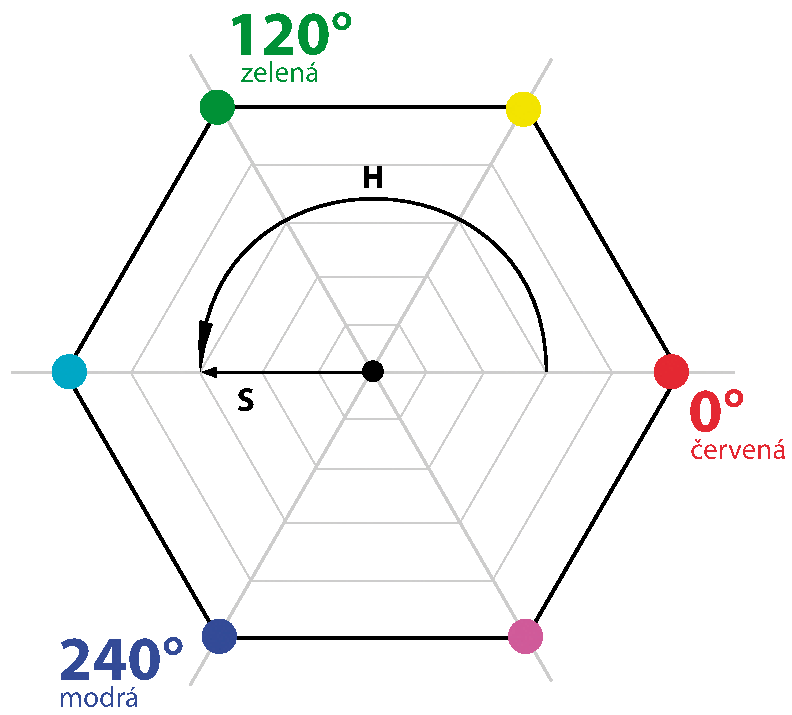
\includegraphics[width=6cm]{figures/hsv}
\caption{Hodnoty HS barevného prostoru HSV}
\label{fig:hsv}
\end{center}
\end{figure}

\indent
Převod do HSV nicméně není bezproblémový. Můžeme si všimnout, že v případě, kdy je vzdálenost od středu (sytost) nulová, není možné určit odstín a taková barva je nedefinovaná. K tomu dochází v případě, že se jedná o odstín šedé. V modelu RGB tak mají dílčí barevné složky stejné hodnoty. Převod nám nejlépe popíše následující pseudokód:

\begin{verbatim}
min         = min(red, green, blue)
max         = max(red, green, blue)

value       = max
saturation  = (max-min)/max

if saturation == 0
    hue = UNDEFINED
else
    diff = max - min
    if max == red
        hue = (green - blue) / diff
    else
    if max == green
        hue = 2 + (blue - red) / diff
    else
    if max == blue
        hue = 4 + (red - green) / diff

    hue = hue * 60
    if hue < 0
        hue = hue + 360
\end{verbatim}

\indent
Lze pozorovat, že při určování odstínu se dělí rozdílem maximální a minimální hodnoty RGB. V případě šedé jsou všechny tři barvy stejné a rozdíl je nulový. V definičním oboru reálných čísel tak není výpočet definován.

\indent
Sytost lze mimo jiné chápat i jako intenzitu nebo čirost dané barvy, jinými slovy ji lze snižovat přidáváním bílé, kdy se barva stává zakalenější. Hodnota V naopak určuje odchylku od černé. Na základě maximální hodnoty RGB se pak určí, v jaké třetině barevného kola se barva nachází. Kterým směrem a o jakou hodnotu se barva posune, se určí rozdílem sousedních barev.

\indent
Převod do černobílé se provádí snížením sytosti na nulu. U barev, které mají jednu RGB složku nulovou a další 255, tedy maximální, dostaneme vždy bílou. Na \ref{fig:hsv} se jedná o barvy na okraji šestiúhelníku. Nevýhodu tohoto přístupu i přes jeho matematickou správnost je, že tak vznikají bílé plochy, které lidské oko vnímá jako vypálené.

\subsection{Rotace a transformace}
\indent
Rotace je v GalleryManageru řešena přes maticové násobení za pomoci matematického rozšíření knihovny Boost::GIL. Nejprve se vygeneruje rotační matice, kterou se vynásobí všechny souřadnice pixelů. Nastává však problém, že rotace probíhá kolem souřadnic [0, 0], tedy dolního-levého rohu a obraz se dostane mimo plátno. Musí se tak nejprve přizpůsobit velikost plátna a výsledek následně i posunout.

\indent
Boost::GIL využívá matic 3x2, které jsou ve skutečnosti maticemi 3x3, kde poslední řádek je vždy [0 0 1], protože veškeré úpravy probíhají ve 2D prostoru. To umožňuje provádět nejen rotaci, ale i translaci pomocí maticového násobení. Stačí tak vygenerovat jednu transformační matici, která se aplikuje na každou souřadnici. Výpočet probíhá následovně:
$$
\begin{bmatrix}
cos\alpha & -sin\alpha & 0 \\
sin\alpha & cos\alpha & 0 \\
0 & 0 & 1
\end{bmatrix}
\begin{bmatrix}
1 & 0 & t_{x} \\
0 & 1 & t_{y} \\
0 & 0 & 1
\end{bmatrix}
\begin{bmatrix}
x \\
y \\
0
\end{bmatrix}
$$

\indent
Hodnoty $t_{x}$ a $t_{y}$ se získávají funkcemi sin a cos na základě toho, jak se každý roh plátna natočil. Výpočet je různý pro každý kvartál rotace.

\indent 
Při transformaci obrazu, tedy změně jeho velikosti, dochází k jeho deformaci. Je tedy třeba vypočítat výslednou barvu každého nového pixelu. K tomu existuje více metod, kde každá má své výhody i nevýhody. GalleryManager využívá bilineárního vzorkování, které dosahuje nejlepších výsledků, jsou-li rozměry výsledného obrazu nejvýše dvakrát menší nebo dvakrát větší. Pro srovnání se vzorkováním dle nejbližšího souseda, kde se vybírá vždy barva nejbližšího pixelu, se zde barvy průměrují, a proto dosahuje výsledný obraz plynulejších přechodů na kontrastních hranách.

\indent
Bilineární vzorkování používá čtyři okolní pixely, jejichž barvu zprůměruje na základě vzdálenosti od výsledného pixelu. Představíme-li si obraz jako mřížku, výsledný pixel bude v poli této mřížky. Nejprve se vypočte na základě velikosti zvětšení obrazu vážený průměr barvy ve směru osy x u horního a dolního páru pixelů. Následně se vypočte vážený průměr těchto dvou hodnot na základě zvětšení ve směru osy y. Váha poměru, na základě které probíhá průměrování pro barvy v rámci výpočetních párů, záleží na koeficientu, kterým se obraz zvětšuje nebo zmenšuje.


%*****************************************************************************
\chapter{Testování}
\noindent
Testování funkčnosti jednotlivých algoritmů probíhalo porovnáním výsledků s existujícími produkty, zejména s programem Adobe Photoshop.

\section{Porovnání úprav s programem Adobe Photoshop}
\subsection{Převod do černobílé a vykreslování obrazu}
\begin{figure}[ht]
\begin{center}
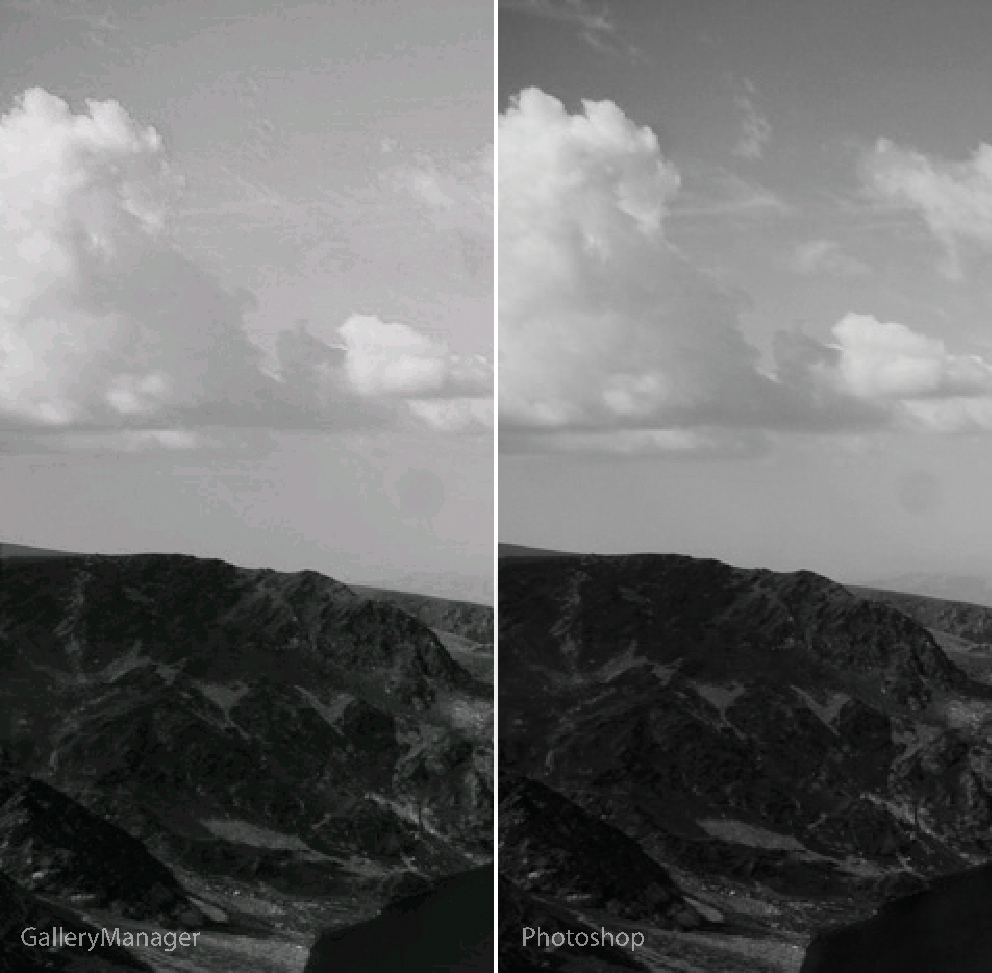
\includegraphics[width=10cm]{figures/bwconvert}
\caption{Převod do černobílé a vykreslování obrazu}
\label{fig:bwconvert}
\end{center}
\end{figure}
\noindent
Na obrázku \ref{fig:bwconvert} si lze všimnout především dvou věcí. První jsou algoritmy, které se používají při automatickém převodu do černobílého prostoru. Fotografie převedená ve Photoshopu má kontrastnější oblohu, než-li fotografie upravená v GalleryManager. Převod na černobílou fotografii se provádí na základě sytosti barev. Syté barvy jsou převedeny na světlé a naopak. Matematicky je sytá barva taková, která má velký rozdíl mezi maximální a minimální hodnotou RGB. Čistá modrá (0, 0, 255), zelená (0, 255, 0) nebo červená (255, 0, 0) budou převedeny na bílou. Lidské oko zároveň vnímá sytost každé barevné složky RGB jinak. Toho využívá Photoshop a nepřevádí lineárně, ale například z modrých, které jsou vnímány jako méně syté, vytváří tmavší barvy. Ze zelených naopak zase barvy světlejší.

\indent
Druhou věcí je vykreslování náhledu obrazu. Photoshop využívá nejspíše i při samotných úpravách antialiasingu\footnote{Vyhlazování hran, oblouky nebo křivky tak nejsou zubaté, ale dodávají zarovnaný dojem} a vyhlazuje tak přechody mezi barvami, u GalleryManageru lze pozorovat stejnobarevné plochy a mezi nimi náhlé tonální skoky.

\subsection{Úprava kontrastu}
\begin{figure}[ht]
\begin{center}
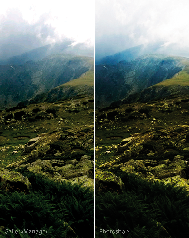
\includegraphics[width=9.5cm]{figures/contrast}
\caption{Úprava kontrastu}
\label{fig:contrast}
\end{center}
\end{figure}

\noindent
Při úpravě kontrastu nabízí Adobe Photoshop dvě možnosti. Novou a starou metodu. Stará metoda funguje stejně jako algoritmus implementovaný v GalleryManageru. Zajímavější je tak porovnat výsledky s novou metodou. Hlavním rozdílem je práce s barvami na hranici bílé. Úprava kontrastu funguje na principu, že čím dále jsou jednotlivé barevné složky od střední šedé (127, 127, 127), tím více danou barevnou složku snížíme, resp. zvýšíme. Extrémně světlé barvy tak začnou nabývat hodnot bílé (255, 255, 255) a tmavé naopak hodnot černé (0, 0, 0). Na \ref{fig:contrast} je toto vidět především na mraku v horní části, kde dochází ke ztrátě kresby. Photoshop se zastaví na minimálních barevných hodnotách a dále už mrakové kontury nezničí.

\indent
Zároveň barvám blíže středu barevného prostoru je přidáváno na sytosti. Tato vlastnost mi nepřijde u Photoshopu příliš dobře zvolená, z fotografického hlediska tak získávají barvy nerealistickou podobu. V GalleryManageru naopak vypadají věrohodněji. Na druhou stranu, Photoshop obsahuje i možnosti úprav jednotlivých barevných kanálů nebo přímo konkrétních odstínů a může tak tyto vlastnosti odstranit jinými způsoby.


\subsection{Úprava sytosti}
\begin{figure}[ht]
\begin{center}
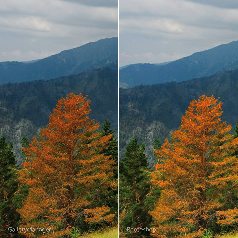
\includegraphics[width=10cm]{figures/saturation}
\caption{Úprava sytosti}
\label{fig:saturation}
\end{center}
\end{figure}

\noindent
Změna sytosti dopadla v obou editorech velice podobně. Ve Photoshopu lze pozorovat, že oranžový strom na obrázku \ref{fig:saturation} v popředí je světlejší, než tomu je u GalleryManageru. Lidské oko vnímá sytost každé barvy trochu jinak. Vnímá tak zelenou nebo i červenou více, než tomu je u modré. GalleryManager bere v úvahu pouze maximální a minimální hodnoty jednotlivých barevných složek. Úpravu sytosti pak provádí lineárně. Photoshop tento fakt bere v úvahu, a tak přisytí některé části fotografie více. Zřetelné to je právě u stromu, kde oranžová obsahuje velké množství zelené a červené, které hodně přispívají k sytosti vnímané lidským okem.

\section{Testování exportu webové prezentace}
\noindent
Vyexportovaná webová prezentace byla otestována přes HTML validator \footnote{http://validator.w3.org/}, který zaručuje, že HTML a CSS kód dodržuje standardy dané konsortiem W3C, a je tak zobrazitelný ve všech dnes používaných webových prohlížečích.


%*****************************************************************************
% Zhodnocení splnění cílů DP/BP a  vlastního přínosu práce (při formulaci je třeba vzít v potaz zadání práce).
% Diskuse dalšího možného pokračování práce.

\chapter{Závěr}

\section{Zhodnocení splnění cílů}
\noindent
Byl vytvořen program GalleryManager, který dává uživateli možnost organizovat a popisovat soubory fotografií. Program dokáže načítat metadata typu EXIF, která jsou vkládána do obrazu každým moderním digitálním fotoaparátem a získat tak všechny důležité údaje o pořízení fotografie (nastavení fotoaparátu - čas, zeměpisná poloha a podobně). 

\indent
Grafický editor umožňuje u fotografií provádět následující úpravy:
\begin{itemize}
\item Úprava jasu a kontrastu
\item Změna sytosti barev
\item Otáčení snímku o libovolný úhel
\item Zmenšování a zvětšování
\item Převod barevné fotografie na černobílou
\end{itemize}
\noindent 
Účinnost zvolených algoritmů byla porovnána s algoritmy používanými programem Adobe Photoshop CS4 za použití testovacích souborů ve formátu JPEG a 8-bitové barevné hloubce. Při použití malých obrazových souborů, které se využívají pro web, je účinnost jednoduchých algoritmů GalleryManageru srovnatelná. Výhody pokročilejších algoritmů používaných ve Photoshopu se projeví při práci s většími soubory a při vícenásobných a rozsáhlejších úpravách snímku. Konkrétní výsledky jsou popsány v sekci testování.

\noindent
Z názvu repositáře na githubu.com (MGalleryManager v2) je patrné, že se jedná o druhou verzi programu. V průběhu práce na první vyšlo najevo, že původní myšlenka napojování jednotlivých modulů na GUI přes datové tabulky způsobovala nedostatek záznamů o provázanosti mezi třídami. Důsledkem bylo, že s každou novou funkcí bylo nutné rozsáhlé přepracování zdrojového kódu.

\indent
Ve druhé verzi je již zcela odděleno uživatelské rozhraní od části programu, která se využívá pro zpracování obrazu. Díky tomu je jednoduché přidávat další funkce, bez rozsáhlých zásahů do celého programu. Aplikaci tak lze snadno rozšiřovat. Kód je volně ke stažení z repositáře na webovém serveru github.com\footnote{https://github.com/macicek/MGalleryManager-v2} a okomentován pomocí syntaxe Doxygen, aby na něm mohli pokračovat i další vývojáři.

\section{Návrhy na zlepšení a cíle do budoucnosti}
\noindent
Každý program se dá vždy vylepšovat a kromě malých změn v podobě přívětivosti uživatelského prostředí lze práci do budoucnosti rozšiřovat následujícími projekty:
\begin{itemize}
\item Grafické úpravy implementovat jako samostatnou knihovnu - rozšíření Boost::GIL, oddělit ji tak jako nezávislý projekt
\item Podpora více-bitových barevných hloubek (16-bit, 32-bit)
\item Podpora dalších formátů používaných ve fotografii, především TIFF, RAW (specifický pro jednotlivé výrobce fotoaparátu)
\item Export do formátu PDF nebo v podobě SQL dotazů pro databáze
\end{itemize}

\indent
Obrovskou výhodou knihovny Boost::GIL, pro zpracování obrazu v různých barevných hloubkách nebo formátech, je způsob, kterým je navržena. Už podle názvu Generic Image Library, je většina funkcí napsána jako template\footnote{česky šablona - datové typy nejsou zadány konkrétně, ale vygenerují se jednotlivé verze funkce na základě toho, s jakými datovými typy je použita}. Umožňuje tak pracovat stejně s 8-bit RGB prostorem jako s 16-bit CMYK. Je třeba implementovat pouze podporu pro jednotlivé formáty a algoritmy pro úpravu obrazu napsat dostatečně genericky, aby mohly pracovat nad libovolným barevným prostorem nebo hloubkou.

\indent
Mělo by se tak navázat na myšlenku generického programování i při implementaci samostatné knihovny pro úpravu obrazu.

\indent
Cílem je zahrnout práci do redakčního systému a navázat ji na databázi rozpracovaných webových serverů FotoAtlas.cz a PhotographicAtlas.com. V oblasti grafických úprav bude přínosem implementovat pokročilejší algoritmus pro zmenšení obrazu, jako například bikubické převzorkování. Aktuálně GalleryManager využívá bilineární převzorkování. Pro uživatele by byla přínosem i ochrana fotografií pomocí individuálních vodoznaků.

\indent
V průběhu svého studia bych se i nadále chtěl věnovat algoritmům pro úpravu obrazu. Rád bych tedy rozšířil práci do podoby samostatného projektu grafické C++ knihovny implementující i pokročilejší algoritmy, než-li jsou použity v GalleryManageru.

% Literatura všeobecně používaná během implementace
\nocite{boostgil}
\nocite{exif}
\nocite{git}
\nocite{libexif}
\nocite{qt}
\nocite{stl}
\nocite{jpeg}
\nocite{wiki:rotation}
\nocite{wiki:affine}
\nocite{wiki:bilinear}
\nocite{wiki:latex}
\nocite{colorhandbook}
\nocite{doxygen}

\bibliography{reference}
\addcontentsline{toc}{chapter}{Literatura}


%*****************************************************************************
% Seznam literatury je v samostatnem souboru reference.bib. Ten
% upravte dle vlastnich potreb, potom zpracujte (a do textu
% zapracujte) pomoci prikazu bibtex a nasledne pdflatex (nebo
% latex). Druhy z nich alespon 2x, aby se poresily odkazy.

% originally following specification for bibliography formating was used
%\bibliographystyle{abbrv}

% Here is an improvment by Petr Dlouhy (April 2010).
% It is mainly for supervisors who expect Czech fomrating rules for references
% Additional feature is live url addresses to sources from your pdf file
% It requires the file csplainnat.bst (included in this sample zipfile).



% M. Dušek radi:
%\bibliographystyle{alpha}
% kdy citace ma tvar [AutorRok] (napriklad [Cook97]). Sice to asi neni  podle ceske normy (BTW BibTeX stejne neodpovida ceske norme), ale je to nejprehlednejsi.
% 3.5.2009 JZ polemizuje: BibTeX neobvinujte, napiste a poskytnete nam styl (.bst) splnujici citacni normu CSN/ISO.

%*****************************************************************************
%*****************************************************************************
\appendix

%*****************************************************************************
\chapter{Seznam použitých zkratek}

\begin{description}
\item[API] Application Programming Interface
\item[CMYK] Cyan Magenta Yellow Black
\item[EXIF] Exchangeable Image File Format
\item[GIL] Generic Image Library
\item[GUI] Graphical User Interface
\item[HSV] Hue Saturation Value
\item[IPTC] Information Interchange Model - International Press Telecommunications Council
\item[IFD] Image File Directory
\item[JPEG] Joint Photographic Experts Group
\item[LGPL] GNU Lesser General Public License
\item[RGB] Red Green Blue
\item[STL] Standard Template Library
\item[TIFF] Tagged Image File Format
\item[W3C] World Wide Web Consortium
\item[XMP] Extensible Metadata Platform

\end{description}
\vdots

%*****************************************************************************
\chapter{Instalační a uživatelská příručka}
\noindent
Na přiloženém CD je k nalezení spustitelný *.exe soubor s přiloženými dynamickými knihovnami pro operační systému Windows. V případě potřeby spustit projekt pod operačním systémem Linux je třeba projekt znovu zkompilovat.

\indent
Projekt je závislý na knihovnách libjpeg, Boost::gil (verze 1.47) s rozšířeními, Qt (verze 4.7) a libexif.

\indent
Při kompilaci pod OS Linux je třeba postupovat následovně:
\begin{enumerate}
\item Nainstalovat knihovnu libjpeg, která je k nalezení na \verb|http://www.ijg.org/|.
\item Stáhnout knihovnu Boost (je otestována na verzi 1.47, u verze 1.48, která vyšla během psaní bakalářské práce, docházelo ke kolizím jmen s knihovnou Qt) . K nalezení je na \verb|http://sourceforge.net/projects/boost/files/boost/1.47.0/|. Knihovna je tvořena hlavičkovými soubory, není tak třeba instalace. Pro GIL je třeba i numerické rozšíření z \verb|http://opensource.adobe.com/wiki/display/gil/Downloads|, které se pouze nakopíruje do stávající knihovny Boost.
\item Nainstalovat knihovnu libexif, která je k nalezení na 
\newline \verb|http://sourceforge.net/projects/libexif/files/libexif/0.6.20/|.
\item Nainstalovat Qt SDK z \verb|http://qt.nokia.com/downloads|.
\item Projekt spustit v prostředí Qt Creator.
\item Je třeba upravit projektový soubor MGalv2.pro, kde se do LIBS přidají odkazy na knihovny libjpeg a libexif a do INCLUDEPATH cesty k hlavičkovým souborům Boost::GIL, libexif a libjpeg.
\item Spustit kompilaci v prostředí Qt Creator.
\end{enumerate}

\indent
Pro instalace knihoven libexif a libjpeg by mělo stačit změnit cestu v konzoli na složku, do které byly knihovny nakopírovány a následně jen spustit příkazy:
\newline ./configure
\newline make
\newline make install

%*****************************************************************************
\chapter{Obsah přiloženého CD}
\noindent
Kromě tohoto dokumentu je na přiloženém CD i program ve spustitelné podobě společně se všemi závislostmi, zdrojové kódy, testovací soubory, z nich vytvořený projekt a z projektu vyexportovaná webová stránka. Struktura CD je následující:
\begin{itemize}
\item /kořenový adrešář
\begin{itemize}
\item \textbf{/exe} - složka obsahující spustitelný program a všechny závislosti
	\begin{itemize}
	\item gallerymanager.exe - spustitelný program
	\item *.dll - dynamické knihovny potřebné ke spuštění programu
	\item \textbf{/images} - složka obsahující obrázky využívané programem
		\subitem *.png - obrázky ve formátu PNG využívané programem
		\subitem *.jpg - obrázky ve formátu JPG využívané programem
	\end{itemize}

\item \textbf{/export} - složka obsahující testovací vyexportovaný projekt z aplikace

\item \textbf{/sample} - složka obsahující testovací fotografie
	\begin{itemize}
	\item \textbf{/musala} - složka obsahující vzorové obrázky
	\subitem *.jpg - vzorové obrázky ve formátu JPG
	\item \textbf{/rilskajezera} - složka obsahující vzorové obrázky
	\subitem *.jpg - vzorové obrázky ve formátu JPG
	\item \textbf{/rilskymonastyr} - složka obsahující vzorové obrázky
	\subitem *.jpg - vzorové obrázky ve formátu JPG		
	\item *.jpg - vzorové obrázky ve formátu JPG
	\end{itemize}
	
\item \textbf{/src} - složka obsahující zdrojové kódy
	\begin{itemize}
	\item \textbf{/core} - složka obsahující cpp/h soubory s třídami jádra, tj. pro práci s fotografiemi a galeriemi
		\subitem *.png - obrázky ve formátu PNG využívané programem
		\subitem *.jpg - obrázky ve formátu JPG využívané programem
	\item \textbf{/gui} - složka obsahující cpp/h soubory s GUI třídami
		\begin{itemize}		
		\item \textbf{/mgridwidget} - složka obsahující cpp/h soubory prvku MGridWidget (část GUI, kde se zobrazuje editor a obsah galerií)			
			\subitem *.cpp - C++ soubory
			\subitem *.h - hlavičkové soubory
		\item \textbf{/mtreewidget} - složka obsahující cpp/h soubory prvku MTreeWidget (část GUI zobrazující stromovou strukturu projektu)
			\subitem *.cpp - C++ soubory
			\subitem *.h - hlavičkové soubory
		\item *.cpp - C++ soubory
		\item *.h - hlavičkové soubory
		\end{itemize}			
	\item MGalv2.pro - projektový soubor editoru Qt Creator
	\item MGalv2.pro.user - uživatelská nastavení projektu
	\item *.cpp - C++ soubory
	\item *.h - hlavičkové soubory
	\end{itemize}
\item \textbf{/text} - složka obsahující dokumentaci k bakalářské práci
	\begin{itemize}
	\item bp.pdf - vyexportovaná práce ve formátu PDF
	\item bp.tex - zdrojový kód dokumentace práce
	\item bp.bbl - zdrojový kód použité literatury
	\item readme.txt - návody ke spuštění a kompilaci programu, technické parametry
	\item \textbf{/figures} - složka obsahující obrázky používané v dokumentaci
	\subitem *.pdf - obrázky ve formátu PDF
	\end{itemize}	
\end{itemize}
\end{itemize}

\end{document}
